\section{Reproducibility}
\only<article>{
  One of the main problems in science is reproducibility: when we are trying to draw conclusions from one specific data set, it is easy to make a mistake. For that reason, the scientific process requires us to use our conclusions to make testable predictions, and then test those predictions with new experiments.}


\begin{frame}
  \frametitle{Reproducibility}
  \only<2>{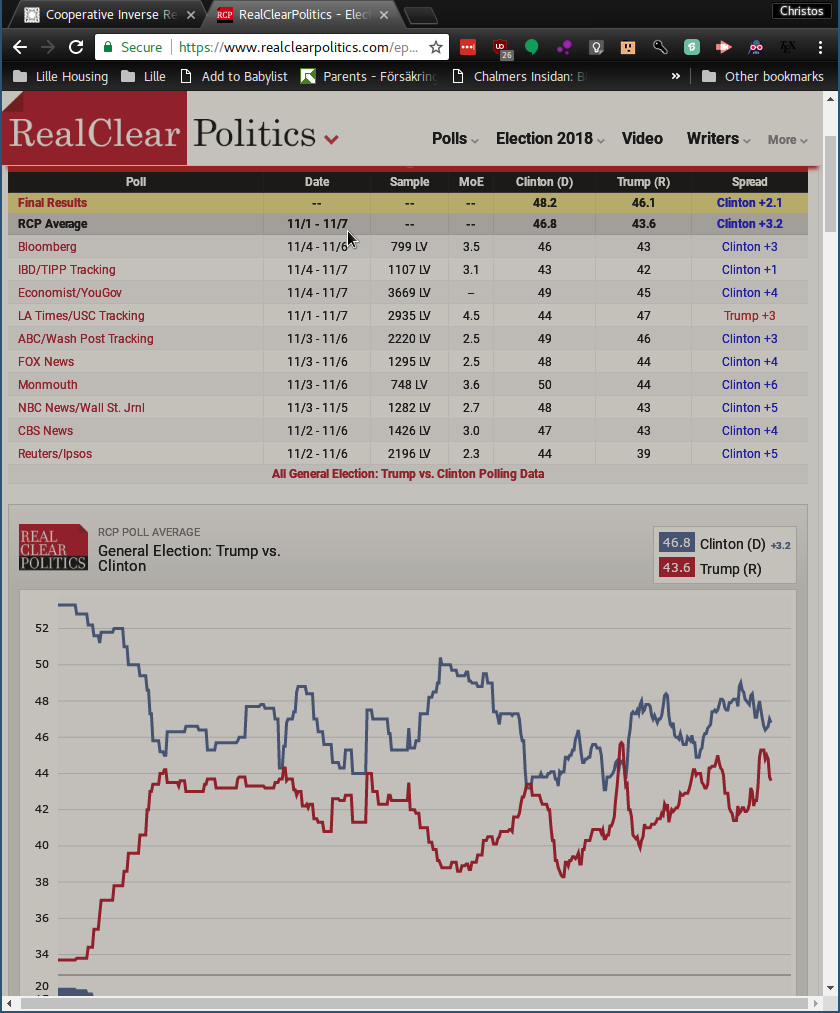
\includegraphics[width=\textwidth]{../figures/2016-election}}
  \only<article>{A simple example is the 2016 election. While we can make models}
  
\end{frame}
\only<article>{The same thing can be done in when dealing purely with data, by making sure we use some of the data as input to the algorithm, and other data to measure the quality of the algorithm itself. In the following, we assume we have some algorithm $\alg : \Datasets \to \CY$, where $\Datasets$ is the universe of possible input data and $\CY$ the possible outputs, e.g. all possible classification rules. We also assume the existence of some quality measure $U$.
}




\begin{frame}
  \begin{figure}[H]
    \begin{center}
      \begin{tikzpicture}[line width=2pt]
        \node<1->[select,label=above:Data Collection] at (0,2) (experiment) {$\chi$};
        \node<3->[select,label=below:{Algorithm, hyperparameters}] at (0,0) (alg) {$\alg$};
        \node<2->[RV,label=above:Training] at (4,2) (training) {$\Training$};
        \node<5->[RV,label=above:Holdout] at (8,2) (holdout) {$\Holdout$};
        \draw<2->[blue,->] (experiment) -- (training);
        \draw<6->[blue,->] (experiment) to [bend left=45] (holdout);
        \node<4->[RV,label=below:Classifier] at (4,0) (pol) {$\pol$};
        \draw<4->[red,->,dashed] (experiment) -- (pol);
        \draw<4->[red,->] (alg) -- (pol);
        \draw<4->[red,->] (training) -- (pol);
        \node<7->[utility,label=below:Measurement] at (8,0) (util) {$\util$};
        \draw<7->[red,->] (pol) -- (util);
        \draw<7->[red,->] (holdout) -- (util);
      \end{tikzpicture}
    \end{center}
    \caption{The decision process in classification.}
  \end{figure}
  \only<article>{One can think of the decision process in classification as follows. First, we decide to collect some data according to some experimental protocol $\chi$. We also decide to use some algorithm (with associated hyperparameters) $\alg$ together with data $\Training$ we will obtain from our data collection in order to obtain a classification policy $\pol$. Typically, we need to measure the quality of a policy according to how well it classifies on unknown data. This is because our policy has been generated using $\Training$, and so any measurement of its accuracy is going to be biased.}
  \uncover<5->{
    \begin{block}{Classification accuracy}
      \[
      \E_\chi[\util(\pol)] = \sum_{x,y} \underset{\textrm{Data probability}}{\underbrace{\Pr_\chi(x, y)}} \overset{\textrm{Decision probability}}{\overbrace{\pol(a = y \mid x)}}
      \]
      \only<article>{The classification accuracy of policy $\poL$ under $\chi$ is the expected number of times the policy decides $\pol$ chooses the correct class.}
    \end{block}
  }
\end{frame}

\begin{frame}
  \frametitle{The human as an algorithm.}
  \only<article>{The same way with which an algorithm creates a model from some prior assumptions and data, so can a human select an algorithm and associated hyperparamters by executing an algorithm herself. This involves trying different algorithms and hyperparametrs on the same training data $\Training$ and then measuring their performance in the holdout set $\Holdout$.}
  \centering
  \begin{tikzpicture}[line width=2pt]
    \node[select,label=above:Data Collection] at (0,2) (experiment) {$\chi$};
    \node[RV,label=above:Training] at (4,2) (training) {$\Training$};
    \node[RV,label=above:Holdout] at (8,2) (holdout) {$\Holdout$};
    \draw[blue,->] (experiment) -- (training);
    \draw[blue,->] (experiment) to [bend left=45] (holdout);
    \node<2->[select,label=below:{Algorithm, hyperparameters}] at (0,0) (alg) {$\alg_1$};     
    \node<3->[RV,label=below:Classifier] at (4,0) (pol) {$\pol_1$};
    \draw<3->[red,->] (alg) -- (pol);
    \draw<3->[red,->] (training) -- (pol);
    \node<4->[utility,label=below:Measurement] at (8,0) (util) {$\util_1$};
    \draw<4->[red,->] (pol) -- (util);
    \draw<4->[red,->] (holdout) -- (util);
    \node<5->[select,label=below:{Algorithm, hyperparameters}] at (0,-2) (alg2) {$\alg_2$};
    \node<6->[RV,label=below:Classifier] at (4,-2) (pol2) {$\pol_2$};
    \node<7->[utility,label=below:Measurement] at (8,-2) (util2) {$\util_2$};
    \draw<6->[red,->] (alg2) -- (pol2);
    \draw<6->[red,->] (training) to [bend left] (pol2);
    \draw<7->[red,->] (pol2) -- (util2);
    \draw<7->[red,->] (holdout) to [bend right] (util2);
  \end{tikzpicture}

\end{frame}

\begin{frame}
  \frametitle{Holdout sets}
  \begin{itemize}
  \item Original data $\Data$, e.g. $\Data = (x_1, \ldots, x_T)$.
  \item Training data $\Training \subset \Data$, e.g. $\Training = x_1, \ldots, x_n$, $n < T$.
  \item Holdout data $\Holdout = D \setminus \Training$, used to measure the quality of the result.
  \item Get algorithm output $y = \alg(\Training)$.
  \item Calculate quality of output $U(y, \Holdout)$
  \end{itemize}
  \only<article>{
    As typically algorithms are maximising the quality metric on the training data, 
    \[
    \alg(\Training) = \argmax_y U(y, \Training)
    \]
    we typically obtain a biased estimate, which depends both on the algorithm itself and the training data. For \KNN{} in particular, when we measure accuracy on the training data, we can nearly always obtain near-perfect accuracy.\footnote{But not always perfect. Can you explain why?}
  }
\end{frame}

\subsection{Algorithmic sensitivity}
\only<article>{The algorithm's output does have a dependence on its input, obviously. So, how sensitive is the algorithm to the input?}
\begin{frame}
  \frametitle{Independent data sets}
  \only<article>{One simple idea is to just collect independent datasets and see how the output of the algorithm changes when the data changes. However, this is quite expensive, as it not might be easy to collect data in the first place.}
  \centering
  \begin{tikzpicture}[line width=2pt]
    \node[select,label=above:Experiment] at (0,0) (experiment) {$\chi$};
    \node[select,label=below:{Algorithm}] at (8,0) (alg) {$\alg$};
    \node[RV,label=below:1st sample] at (4,0) (sample1) {$D_1$};
    \node[RV,label=below:1st Result] at (6,0) (pol1) {$\pol_1$};
    \node<2>[RV,label=above:2nd Sample] at (4,2) (sample2) {$D_2$};
    \node<2>[RV,label=above:2nd Result] at (6,2) (pol2) {$\pol_2$};
        \draw[blue,->] (experiment) -- (sample1);
    \draw[red,->] (alg) -- (pol1);
    \draw[red,->] (sample1) -- (pol1);
    \draw<2>[blue,->] (experiment) -- (sample2);
    \draw<2>[red,->] (alg) -- (pol2);
    \draw<2>[red,->] (sample2) -- (pol2);
  \end{tikzpicture}
\end{frame}
\begin{frame}
  \frametitle{Bootstrap samples}
  \only<article>{A more efficient idea is to only collect one dataset, but then use it to generate more datasets. The simplest way to do that is by sampling with replacement from the original dataset, new datasets of the same size as the original. Then the original dataset is sufficiently large, this is approximately the same as sampling independent datasets.}
  \centering
  \begin{tikzpicture}[line width=2pt]
    \node[select,label=above:Experiment] at (0,0) (experiment) {$\chi$};
    \node[RV,label=below:training] at (2,0) (training) {$\Training$};
    \draw[blue,->] (experiment) -- (training);
    \node[select,label=below:{Algorithm}] at (8,0) (alg) {$\alg$};
    \node[RV,label=below:1st sample] at (4,0) (sample1) {$D_1$};
    \node[RV,label=below:1st Result] at (6,0) (pol1) {$\pol_1$};
    \node<2>[RV,label=above:2nd Sample] at (4,2) (sample2) {$D_2$};
    \node<2>[RV,label=above:2nd Result] at (6,2) (pol2) {$\pol_2$};
    \draw[red,->] (alg) -- (pol1);
    \draw[red,->] (sample1) -- (pol1);
    \draw[red,->] (training) -- (sample1);
    \draw<2>[red,->] (training) -- (sample2);
    \draw<2>[red,->] (alg) -- (pol2);
    \draw<2>[red,->] (sample2) -- (pol2);
  \end{tikzpicture}
  \only<article>{As usual, we can evaluate our algorithm on an independent holdout set.}
\end{frame}



\begin{frame}
  \frametitle{Bootstrapping}
  Bootstrapping is a general technique that can be used to.
  \begin{itemize}
  \item Estimate the sensitivity of $\alg$ to the data $x$
  \item Obtain a distribution of estimates $y$ from $\alg$ and the data $x$.
  \end{itemize}
  \begin{block}{Bootstrapping}
    \begin{itemize}
    \item \textbf{Input} Training data $\Training$, number of samples $k$.
    \item \textbf{For} $i = 1, \ldots, k$
    \item \quad $\Data^{(i)} = \textrm{Bootstrap}(\Training)$
    \item \quad $y_i = \alg(\Data^{(i)})$
    \item \textbf{return} $\{y_1, \ldots, y_i\}$.
    \end{itemize}
    where  $\textrm{Bootstrap}(\Training)$ samples with replacement $|\Training|$ points.
  \end{block}

\end{frame}
\only<article>{
  In general, it is worthwhile to have some indication of how certain we should be about our prediction. Bayesian inference offers a principled way to do this.
}




\subsection{Bayesian credible intervals}


\subsection{Model mismatch}

\subsection{Boot-strapping}

\subsection{Cross-validation}

\subsection{Independent replication}



%%% Local Variables:
%%% mode: latex
%%% TeX-master: "notes"
%%% End:

